% This file was created by matlab2tikz v0.4.7 running on MATLAB 8.4.
% Copyright (c) 2008--2014, Nico Schlömer <nico.schloemer@gmail.com>
% All rights reserved.
% Minimal pgfplots version: 1.3
% 
% The latest updates can be retrieved from
%   http://www.mathworks.com/matlabcentral/fileexchange/22022-matlab2tikz
% where you can also make suggestions and rate matlab2tikz.
% 
\documentclass[tikz]{standalone}
\usepackage{pgfplots}
\usepackage{grffile}
\pgfplotsset{compat=newest}
\usetikzlibrary{plotmarks}
\usepackage{amsmath}

\begin{document}
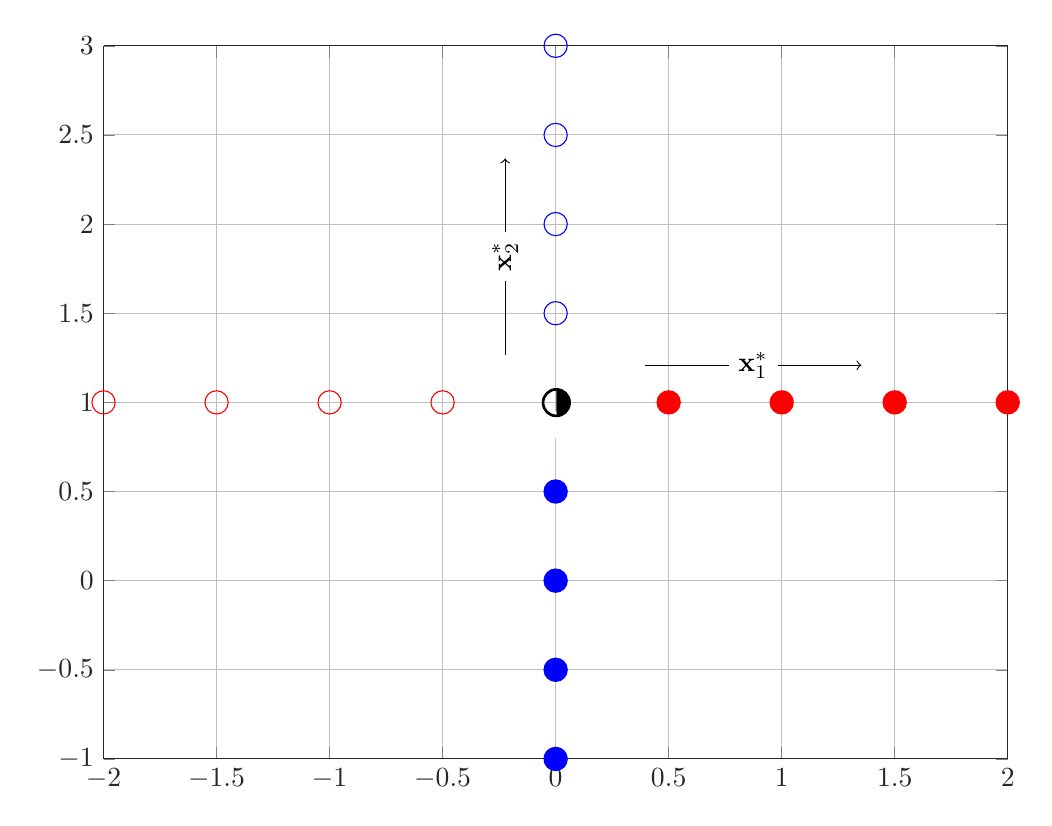
\begin{tikzpicture}

\begin{axis}[%
width=4.52083333333333in,
height=3.565625in,
scale only axis,
separate axis lines,
every outer x axis line/.append style={white!15!black},
every x tick label/.append style={font=\color{white!15!black}},
xmin=-2,
xmax=2,
xmajorgrids,
every outer y axis line/.append style={white!15!black},
every y tick label/.append style={font=\color{white!15!black}},
ymin=-1,
ymax=3,
ymajorgrids
]
\addplot [color=blue,mark size=4.2pt,only marks,mark=*,mark options={solid},forget plot]
  table[row sep=crcr]{0	-1\\
};
\addplot [color=red,only marks,mark size=4.2pt,mark=o,mark options={solid},forget plot]
  table[row sep=crcr]{-2	1\\
};
\addplot [color=blue,mark size=4.2pt,only marks,mark=*,mark options={solid},forget plot]
  table[row sep=crcr]{0	-0.5\\
};
\addplot [color=red,only marks,mark size=4.2pt,mark=o,mark options={solid},forget plot]
  table[row sep=crcr]{-1.5	1\\
};
\addplot [color=blue,mark size=4.2pt,only marks,mark=*,mark options={solid},forget plot]
  table[row sep=crcr]{0	0\\
};
\addplot [color=red,only marks,mark size=4.2pt,mark=o,mark options={solid},forget plot]
  table[row sep=crcr]{-1	1\\
};
\addplot [color=blue,mark size=4.2pt,only marks,mark=*,mark options={solid},forget plot]
  table[row sep=crcr]{0	0.5\\
};
\addplot [color=red,only marks,mark=o,mark size=4.2pt,mark options={solid},forget plot]
  table[row sep=crcr]{-0.5	1\\
};
%\addplot [color=black,mark size=4.2pt,only marks,mark=halfcircle,mark options={solid},forget plot]
%  table[row sep=crcr]{0	1\\
%};
\addplot [color=blue,only marks,mark size=4.2pt,mark=o,mark options={solid},forget plot]
  table[row sep=crcr]{0	1.5\\
};
\addplot [color=red,mark size=4.2pt,only marks,mark=*,mark options={solid},forget plot]
  table[row sep=crcr]{0.5	1\\
};
\addplot [color=blue,only marks,mark size=4.2pt,mark=o,mark options={solid},forget plot]
  table[row sep=crcr]{0	2\\
};
\addplot [color=red,mark size=4.2pt,only marks,mark=*,mark options={solid},forget plot]
  table[row sep=crcr]{1	1\\
};
\addplot [color=blue,only marks,mark size=4.2pt,mark=o,mark options={solid},forget plot]
  table[row sep=crcr]{0	2.5\\
};
\addplot [color=red,mark size=4.2pt,only marks,mark=*,mark options={solid},forget plot]
  table[row sep=crcr]{1.5	1\\
};
\addplot [color=blue,only marks,mark size=4.2pt,mark=o,mark options={solid},forget plot]
  table[row sep=crcr]{0	3\\
};
\addplot [color=red,mark size=4.2pt,only marks,mark=*,mark options={solid},forget plot]
  table[row sep=crcr]{2	1\\
};
\end{axis}

\node [rotate=-90, scale=2.4, text=black] at (5.75, 4.525) {\pgfuseplotmark{halfcircle*}};

\node(n1)       at (6.75,5)    {};
\node(n2)       at (9.75,5)    {};
% this path will place/draw a node call (text)
\path (n1) -- node[sloped] (text) {$\mathbf{x}_1^*$} (n2);
% Now draw arrows. This way it will be like you want.
\draw[->] (n1)--(text)--(n2);
% If you use two draw commands, will get two arrows.
%\draw[->] (n1)--(text);
%\draw[->] (text)--(n2);


\node(n1)       at (5.1,5)    {};
\node(n2)       at (5.1,7.75)    {};
% this path will place/draw a node call (text)
\path (n1) -- node[sloped] (text) {$\mathbf{x}_2^*$} (n2);
% Now draw arrows. This way it will be like you want.
\draw[->] (n1)--(text)--(n2);
% If you use two draw commands, will get two arrows.
%\draw[->] (n1)--(text);
%\draw[->] (text)--(n2);


\end{tikzpicture}%
\end{document}